\documentclass[12pt]{article}
\usepackage[margin=1in]{geometry}
\usepackage{setspace}
\onehalfspacing

% Start of preamble
%==========================================================================================%
% Required to support mathematical unicode
\usepackage[warnunknown, fasterrors, mathletters]{ucs}
\usepackage[utf8x]{inputenc}

\usepackage[dvipsnames,table,xcdraw]{xcolor}

% Standard mathematical typesetting packages
\usepackage{amsmath,amssymb,amscd,amsthm,amsxtra}
\usepackage{mathtools,mathrsfs,xparse}

% fonts
\usepackage{newtxtext, newtxmath}

% Symbol and utility packages
\usepackage{cancel, textcomp}
\usepackage[mathscr]{euscript}
\usepackage[nointegrals]{wasysym}
\usepackage{apacite}

% Extras
\usepackage{physics}  
\usepackage{tikz-cd} 
\usepackage{microtype}
\usepackage{enumitem}
\usepackage{titling}
\usepackage{graphicx}

% Fancy theorems due to @intuitively on discord
\usepackage{mdframed}
\newmdtheoremenv[
backgroundcolor=NavyBlue!30,
linewidth=2pt,
linecolor=NavyBlue,
topline=false,
bottomline=false,
rightline=false,
innertopmargin=10pt,
innerbottommargin=10pt,
innerrightmargin=10pt,
innerleftmargin=10pt,
skipabove=\baselineskip,
skipbelow=\baselineskip
]{mytheorem}{Theorem}

\newenvironment{theorem}{\begin{mytheorem}}{\end{mytheorem}}

\newtheorem{corollary}{Corollary}
\newtheorem{lemma}{Lemma}

\newtheoremstyle{definitionstyle}
{\topsep}%
{\topsep}%
{}%
{}%
{\bfseries}%
{.}%
{.5em}%
{}%
\theoremstyle{definitionstyle}
\newmdtheoremenv[
backgroundcolor=Violet!30,
linewidth=2pt,
linecolor=Violet,
topline=false,
bottomline=false,
rightline=false,r
innertopmargin=10pt,
innerbottommargin=10pt,
innerrightmargin=10pt,
innerleftmargin=10pt,
skipabove=\baselineskip,
skipbelow=\baselineskip,
]{mydef}{Definition}
\newenvironment{definition}{\begin{mydef}}{\end{mydef}}

\newtheorem*{remark}{Remark}

\newtheorem*{example}{Example}

% Common shortcuts
\def\mbb#1{\mathbb{#1}}
\def\mfk#1{\mathfrak{#1}}

\def\bN{\mbb{N}}
\def \C{\mbb{C}}
\def \R{\mbb{R}}
\def\bQ{\mbb{Q}}
\def\bZ{\mbb{Z}}
\def \cph{\varphi}
\renewcommand{\th}{\theta}
\def \ve{\varepsilon}
\newcommand{\mg}[1]{\| #1 \|}

% Often helpful macros
\newcommand{\floor}[1]{\left\lfloor#1\right\rfloor}
\newcommand{\ceil}[1]{\left\lceil#1\right\rceil}
\renewcommand{\qed}{\hfill\qedsymbol}
\renewcommand{\P}{\mathbb P\qty}
\newcommand{\E}{\mathbb{E}\qty}
\newcommand{\Cov}{\mathrm{Cov}\qty}
\newcommand{\Var}{\mathrm{Var}\qty}
\renewcommand{\ip}[1]{\langle #1 \rangle}

% Sets
\usepackage{braket}

\graphicspath{{/}}
\usepackage{float}

\newcommand{\SET}[1]{\Set{\mskip-\medmuskip #1 \mskip-\medmuskip}}

% End of preamble
%==========================================================================================%

% Start of commands specific to this file
%==========================================================================================%

\usepackage{listings}
\lstset{
    basicstyle=\ttfamily,
    breaklines=true,
    frame=single,
    backgroundcolor=\color{gray!10},
    keywordstyle=\color{blue},
    commentstyle=\color{gray}
}

%==========================================================================================%
% End of commands specific to this file

\title{CSE 422 HW5}
\date{\today}
\author{Rohan Mukherjee}

\begin{document}
    \maketitle
    \begin{enumerate}[leftmargin=\labelsep]
        \item \textbf{Image Compression}
        \begin{enumerate}[label=\textbf{(\alph*)}]
            \item Some matrices can't immediately be interpreted as images since they might have values outside of $[0,255]$. My solution was to just clamp the resulting matrix values into this range.
            
            Here is the picture of the rank-k approximation of the image for different $k$s:
            \begin{figure}[H]
                \centering
                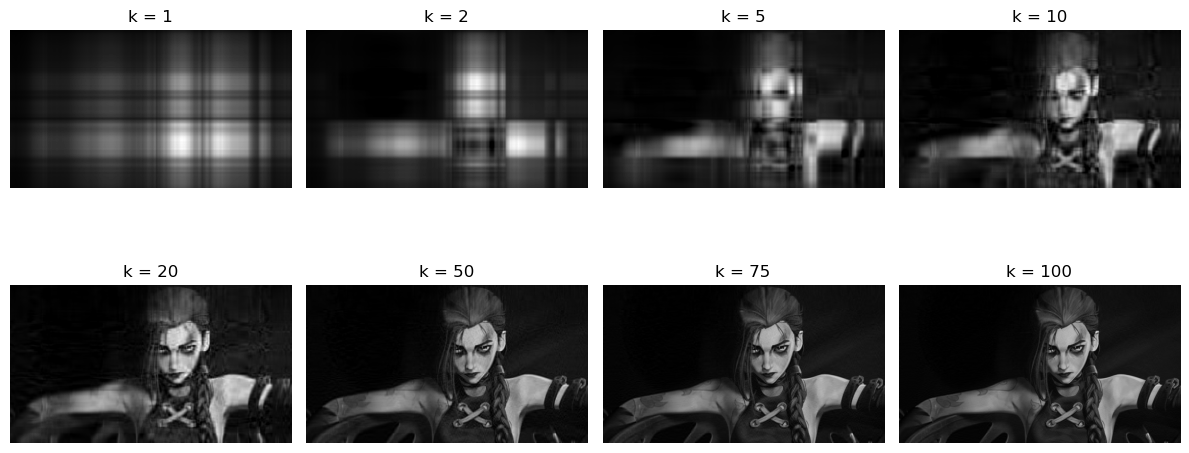
\includegraphics[width=\textwidth]{rank_k_approx.png}
                \caption{Rank-k approximation of the image}
            \end{figure}
    
            \item Since the image is a $563\times 1000$ matrix, it has rank at most 563. So there are at very most 563 non-zero singular values, so a rank 563 SVD is prescisely the image.
    
            \item Here is a picture of the first left/right singular vectors, plotted against the column/row average:
            \begin{figure}[H]
                \centering
                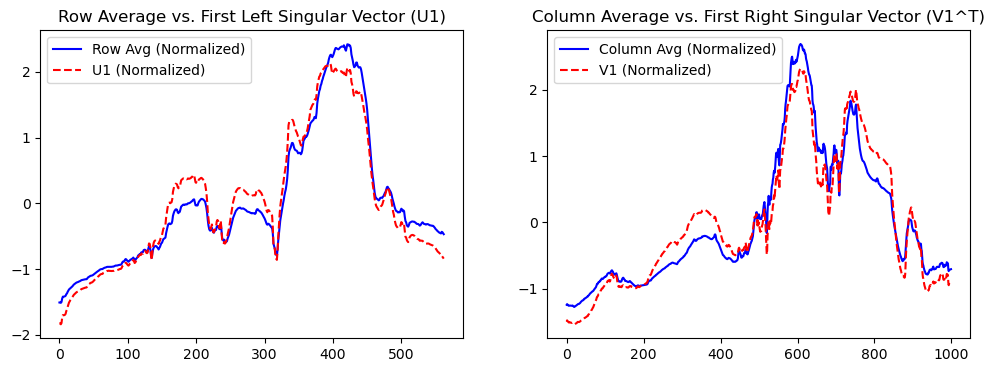
\includegraphics[width=0.8\textwidth]{left_and_right_sing.png}
                \caption{First left/right singular vectors plotted against the column/row average}
            \end{figure}
            As you can see, these are almost the same thing. The first left/right singular vectors very closely approximate the column/row average of the image. This is of course what I would've expected since it would make sense that the best rank-1 approximation should be some sort of average.
    
            \item Recall that an SVD of $M \in \R^{m \times n}$ is $M = U \Sigma V^T$, where $U$ is $m \times m$, $\Sigma$ is $m \times n$ and $V$ is $n \times n$. So if we had a rank-k approximation, we would need to store the $k$ singular values, the $m \times k$ matrix $U$ and the $k \times n$ matrix $V$. This takes a total of $m \times k + k + k \times n = mk + kn + k$ bytes, which is $O(k(m+n))$. In the above image, at least for me, the $k=50$ approximation looks almost indistinguishable from the real image. A $k=50$ approximation thus takes approximately $50 \times (563 + 1000) = 50 \times 1563 = 78150$ bytes, which is a 7x savings from $563 \times 1000 = 563000$ bytes needed to store the original image. The $k=100$ approximation is thus around a 3.5x savings.
    
            \item For very small values of $k$, we can see a lot of blurring. In computer vision, I learned that the blurring filter is really just a moving average. From what we discussed above, the first singular vectors are column and row averages. So we will see a lot of blurring since that's just what averages look like. Also, there seems to be some blockiness and color banding, comparing 50 vs 100 from close up. The colors on her left (our right) shoulder are much more well defined and separable in the 100 case vs the 50 case. Her hair, which is notoriously difficult for computer applications to render, also looks blurry. The next few singular vectors are probably some kind of averages too, but when you put a lot of them together it looks great. This process basically turns our image into low resolution, which is why we see some of this blockiness/color banding. 
        \end{enumerate}
        \item \textbf{Word Embeddings}
        \begin{enumerate}[label=\textbf{(\alph*)}]
            \item Here is a plot of the eigenvalues of $\hat M$ in decreasing order:
            \begin{figure}[H]
                \centering
                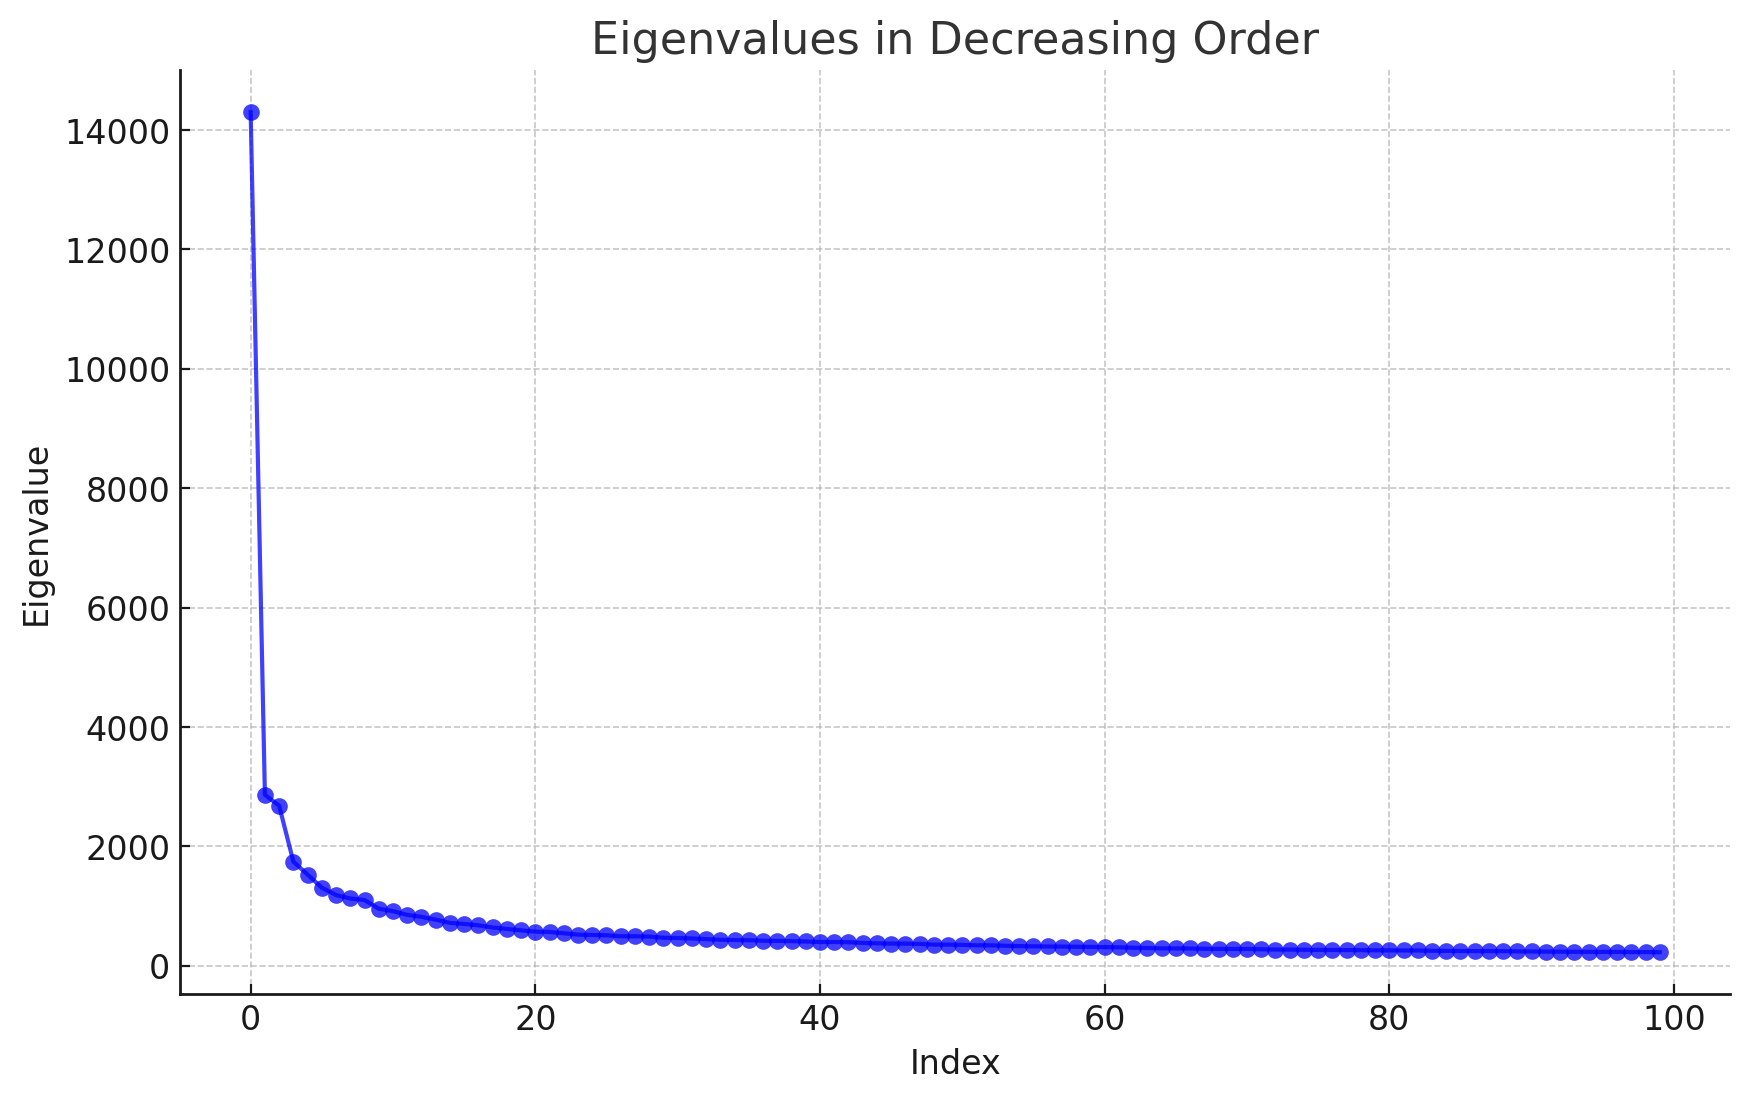
\includegraphics[width=0.8\textwidth]{eigvals_dec_order.png}
                \caption{Eigenvalues of $\hat M$ in decreasing order}
            \end{figure}
            As we can see, we have a dropoff from the first eigenvalue being 14,000 to the second being 2,000, the another large dropoff from 2682 to 1745. Clearly, this graph shows the image is very well approximated by the first few eigenvectors. So I would say its low rank.

            \item Here are 6 interesting singular vectors and their corresponding strongest words:
            \begin{lstlisting}
#1 singular vector most influential words:  
['the', 'and', 'of', 'in', 'to', 'for', 'as', 'is', 'with', 'was']
                \end{lstlisting}

                It looks like the first eigenvector measures if you are an article.
                
                \begin{lstlisting}
#3 singular vector most influential words:  
['born', 'john', 'james', 'david', 'robert', 'william', 'jr', 'george', 'thomas', 'michael']
                
                \end{lstlisting}

                Outside of the weird 'born', it seems like the third eigenvector measures if you are a (male) name.
                
                \begin{lstlisting}
#6 singular vector most influential words:  
['troops', 'digital', 'science', 'software', 'technology', 'engineering', 'him', 'computer', 'research', 'online']
                
                \end{lstlisting}

                These seem to measure if you are a technology word (it is interesting that 'him' shows up in the list of the 10 biggest words, I am wondering if this is related to how the distribution of tech workers is skewed towards men).
                
                \begin{lstlisting}
#7 singular vector most influential words:  
['ancient', 'medieval', 'century', 'greek', 'culture', 'latin', 'poetry', 'literature', 'folk', 'contemporary']
                
                \end{lstlisting}

                These look like words that describe history.
                
                \begin{lstlisting}
#10 singular vector most influential words: 
['ii', 'commander', 'german', 'de', 'iii', 'squadron', 'mm', 'aircraft', 'iv', 'community']
                
                \end{lstlisting}

                These are words that describe WWII.
                
                \begin{lstlisting}
#17 singular vector most influential words:  
['republican', 'democratic', 'conservative', 'at', 'her', 'anti', 'election', 'paris', 'she', 'maria']
                
                \end{lstlisting}

                These are political words (it is again interesting that 'her' and 'she' show up here).

                PCA measures the direction of greatest variance. With our starting assumption that a word is described by its context, we would expect the most variance to be in the direction of the semantics that humans usually use. For example, articles are used in an extremely different context, than names. Names come at the start of a sentence usually and articles are words that go in between two other words. So it makes sense that the eigenvectors would have some measure of semantics. There are of course eigenvectors which aren't interporable, such as:
                \begin{lstlisting}
#4 singular vector most influential words: 
['district', 'you', 'county', 'album', 'council', 'love', 'university', 'me', 'national', 'my']
                \end{lstlisting}

                \item Here is a picture of the projections of the words onto $u = u_1-u_2$ where $u_1$ is th embedding of woman and $u_2$ is the embedding of man:
                \begin{figure}[H]
                    \centering
                    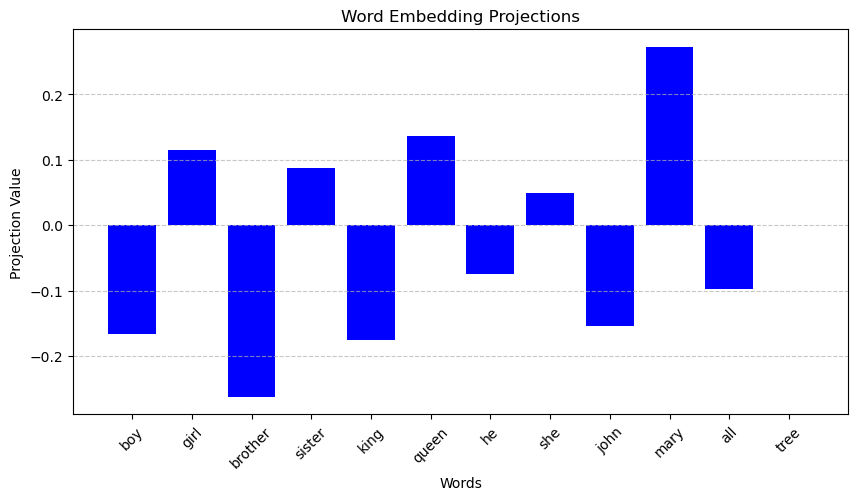
\includegraphics[width=0.8\textwidth]{man_woman_projs.png}
                    \title{Projections of the words onto $u = u_1-u_2$}
                \end{figure}
                Who would've thought. Tree is orthogonal to what makes a man into a woman. This is a telling picture: you would expect brother = sister + (man - woman), which is why it has a really strong negative inner product with woman - man. It is also able to tell "gender" of the name Mary and John using this same logic, since John = Mary + (brother - sister), and Mary = John + (sister - brother). Similarly, we would expect that king = queen + (brother - sister) and queen = king + (sister - brother), and we do indeed get those inner products. 
                
                \item Here is a similar plot for those job words:
                \begin{figure}[H]
                    \centering
                    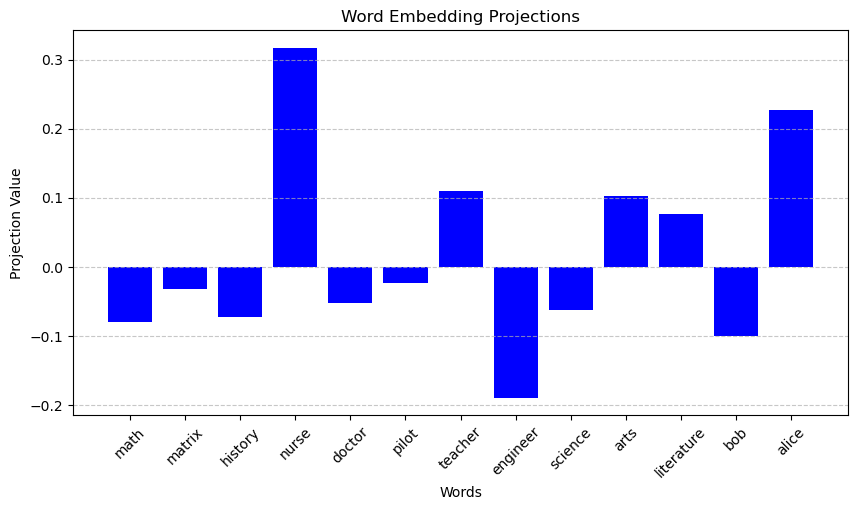
\includegraphics[width=0.8\textwidth]{job_words.png}
                    \title{Projections of the words onto $u = u_1-u_2$}
                \end{figure}
                 The implication is that 'nurse' is a more woman job and 'engineer' is a more man job, based off its correlation with woman-man. Although weaker, it thinks literature, arts, teacher and teacher are more woman jobs, and math, matrix, history, doctor, pilot, and science are more man jobs. It also thinks that bob is a more masculine name and alice is a more feminine one. 
                
                 This is problematic because woman - man, has a really strong positive correlation with nurse, and a really strong negative correlation with engineer. If we trained an NLP model on wikipiedia data, and then used it to recommend successful hires, it would recommend more men than woman based off of this data, since it thinks that more men are engineers than woman. Vice versa, it would recommend more woman than men to be nurses.

                 \item Because we normalized the rows of $U$, which is a 10,000 $\times$ 100 matrix, where word $i$ has embedding into $\R^{100}$ given by $U[i]$, the norm of each row is 1. In particular, $\text{similarity}(w_i,w_j) = \ip{w_i, w_j} / \mg{w_i}\mg{w_j} = \ip{w_i,w_j}$, so this definition corresponds with our usual definition of similarity.

                 The 10 most similar words to `washington' I found were:
                 \begin{lstlisting}
['boston', 'chicago', 'york', 'houston', 'philadelphia', 'baltimore', 'kansas', 'texas', 'florida', 'michigan']
                 \end{lstlisting}

                 The accuracy of the dataset analogy\_tasks.txt I got was 0.549 (I told the analogy finder that it couldn't output a1, a2 or b1 when we are asking for a1:a2::b1:b2, as I saw that happening a lot but it isn't realistic). This is extremely impressive, since it has like 10,000 words to choose from and gets the right word, which would randomly happen with probability $10^{-4}$, 1/2 of the time. It is more than 3 orderes of magnitude better than random.

                 This approach has a few challenges. For starters, something like this:
                 \begin{lstlisting}
#3530 india:indian::ukraine:ukrainian got romanian
#3533 india:indian::brazil:brazilian got mexican
#3535 india:indian::chile:chilean got mexican
#3537 india:indian::croatia:croatian got romanian
#3538 india:indian::denmark:danish got swedish
                 \end{lstlisting}
                 As you can see, the answers it gives are not too wildly off. It gives countries that are reasonably similar, like Ukraine and Romania. I would suspect that this is due to romanian and ukranian having very similar contexts. So it will output something that is reasonable, but might not get the correct answer. We can see this with not just countries:
                 \begin{lstlisting}
#2291 simple:simpler::fast:faster got slower
                 \end{lstlisting}
                 Again, faster and slower have really similar contexts, so they are very similar words. simple vs simpler captures adjective vs adverb, but it does not capture any semantic knowledge about being fast or slow. So it will simply pick an adverb that has similar context to faster. Sometimes this is `faster' but in our case this is `slower'. 

                 You can see this happening again with:
                 \begin{lstlisting}
#4294 jumping:jumped::decreasing:decreased got risen
                 \end{lstlisting}

                 However, sometimes it is just plain wrong. No feasible explanation for why. Like this:
                 \begin{lstlisting}
#5014 dollar:dollars::man:men got woman
#5018 dollar:dollars::woman:women got man
                 \end{lstlisting}
                 This is the most curious result I found. 

                 It can also just get the tense wrong:
                 \begin{lstlisting}
#5579 write:writes::sing:sings got sang
                 \end{lstlisting}

                 It also really struggles with adverbs. For example:
                 \begin{lstlisting}
#1535 apparent:apparently::complete:completely got actually
#1536 apparent:apparently::free:freely got actually
#1537 apparent:apparently::immediate:immediately got reportedly
#1538 apparent:apparently::most:mostly got quite
#1542 apparent:apparently::precise:precisely got supposedly
#1543 apparent:apparently::professional:professionally got already
#1544 apparent:apparently::quick:quickly got surprisingly
#1545 apparent:apparently::rapid:rapidly got initially
#1546 apparent:apparently::rare:rarely got reportedly
#1547 apparent:apparently::safe:safely got supposedly
#1548 apparent:apparently::serious:seriously got reportedly
#1549 apparent:apparently::slow:slowly got too
#1550 apparent:apparently::sudden:suddenly got reportedly
#1551 apparent:apparently::typical:typically got essentially
#1552 apparent:apparently::usual:usually got essentially
#1553 complete:completely::free:freely got totally
#1554 complete:completely::immediate:immediately got totally
#1555 complete:completely::most:mostly got totally
#1556 complete:completely::obvious:obviously got totally
#1557 complete:completely::occasional:occasionally got totally
#1558 complete:completely::possible:possibly got totally
#1559 complete:completely::precise:precisely got totally
#1560 complete:completely::professional:professionally got entirely
#1561 complete:completely::quick:quickly got totally
#1562 complete:completely::rapid:rapidly got totally
#1563 complete:completely::rare:rarely got totally
#1564 complete:completely::safe:safely got totally
#1565 complete:completely::serious:seriously got totally
#1567 complete:completely::sudden:suddenly got totally
#1568 complete:completely::typical:typically got entirely
#1569 complete:completely::usual:usually got totally
#1570 complete:completely::apparent:apparently got totally
                 \end{lstlisting}
                 Lots of `totally'. This might be related to adverbs having different context to their adjectives. For example, we might say `it is apparent that', to emphasize that something is really true. However, `apparently' has a very different meaning, almost questioning if the result is right. So it gets confused and outputs totally.
        \end{enumerate}
    \end{enumerate}
\end{document}